% ============================================================================
% CHAPTER 4 — NN-SCF: NEURAL NETWORK-BASED SCF FOR JOINT PAPR AND BER
% ============================================================================
\chapter{NN-SCF: Joint PAPR Reduction and Signal Recovery}
\label{ch:nn_scf}

\begin{motivation}
    PRNet showed that a neural network can reduce PAPR, but it treats the
    problem in a somewhat ``black-box'' fashion.
    What if we could design a DNN framework that more explicitly separates
    the \emph{PAPR reduction module} from the \emph{signal recovery module},
    and jointly optimizes both with a tunable trade-off?
    Zou et al.\ (2021) proposed the \textbf{Neural Network-based Signal
    Cancellation Framework (NN-SCF)}, which decomposes the problem into
    a PAPR reduction front-end and a signal recovery back-end, connected
    through a multi-objective loss function~\cite{zou2021novel}.
\end{motivation}


% ----------------------------------------------------------------------------
\section{Conceptual Overview}
\label{sec:nnscf_concept}
% ----------------------------------------------------------------------------

The NN-SCF framework approaches PAPR reduction from a \textbf{signal
cancellation} perspective rather than an autoencoder perspective.
The key idea is~\cite{zou2021novel}:

\begin{enumerate}
    \item A \textbf{PAPR reduction module} (DNN) generates a
          \textbf{peak-cancelling signal} $\bm{c}$ that, when added to the
          original OFDM signal $\bm{x}$, reduces the peaks:
          \begin{equation}
              \bm{s} = \bm{x} + \bm{c},
              \label{eq:nnscf_transmission}
          \end{equation}
          where $\bm{s}$ is the transmitted signal with reduced PAPR.

    \item A \textbf{signal recovery module} (another DNN) at the receiver
          estimates and removes the cancellation signal to recover the
          original data:
          \begin{equation}
              \hat{\bm{x}} = \bm{r} - \hat{\bm{c}},
              \label{eq:nnscf_recovery}
          \end{equation}
          where $\bm{r}$ is the received noisy signal and $\hat{\bm{c}}$
          is the estimated cancellation signal.
\end{enumerate}

\begin{figure}[H]
    \centering
    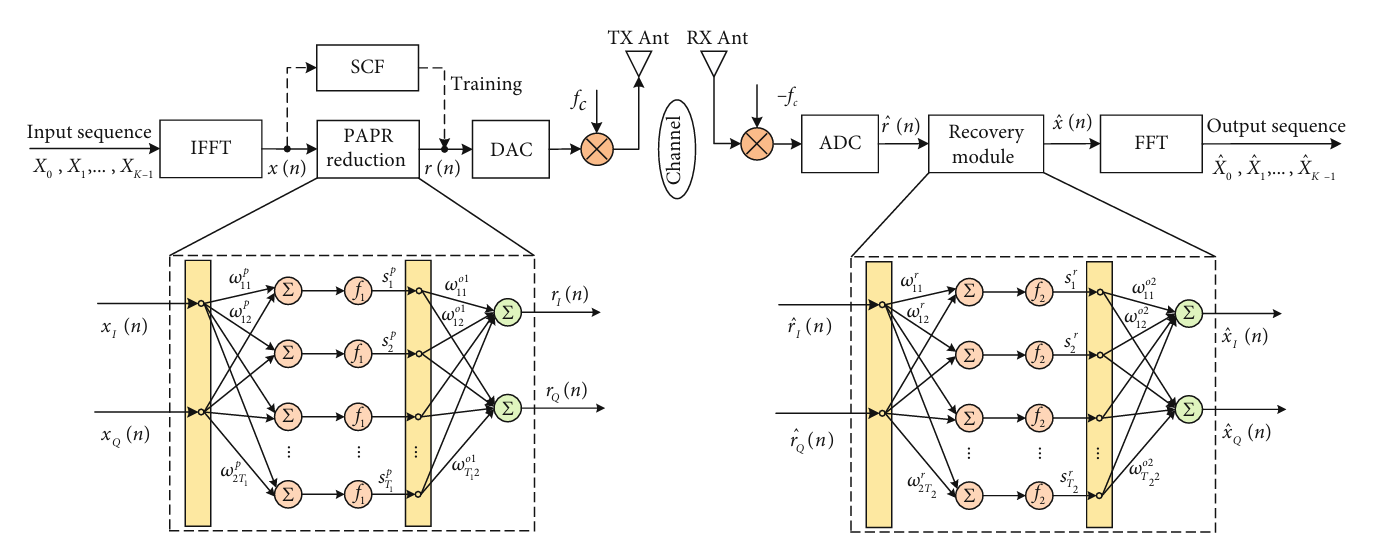
\includegraphics[width=0.95\linewidth]{Figures/16_nn_scf_framework.png}
    \caption{Block diagram of the NN-SCF framework.
             The PAPR reduction module generates a cancellation signal $\bm{c}$
             added to the OFDM signal.  The recovery module at the receiver
             estimates and removes $\bm{c}$ to retrieve the original data.
             Both modules are DNNs trained jointly.
             Reproduced from~\cite{zou2021novel}.}
    \label{fig:nnscf_framework}
\end{figure}

\begin{keyinsight}
    The ``signal cancellation'' framing has a major conceptual advantage:
    the cancellation signal $\bm{c}$ is interpretable---it is literally the
    signal that needs to be subtracted from the peaks.  This is more
    transparent than the PRNet approach, where the encoder's output is an
    opaque nonlinear transformation of the input~\cite{zou2021novel}.
\end{keyinsight}


% ----------------------------------------------------------------------------
\section{System Model and Architecture}
\label{sec:nnscf_architecture}
% ----------------------------------------------------------------------------

\subsection{PAPR Reduction Module}

The PAPR reduction module is a fully connected DNN that maps the $2N$-dimensional
real-valued input (real and imaginary parts of the OFDM signal after IFFT)
to a $2N$-dimensional cancellation signal~\cite{zou2021novel}:
\begin{equation}
    \bm{c} = \mathcal{N}_{\mathrm{Tx}}\!\bigl(\bm{x};\;\bm{\theta}_{\mathrm{Tx}}\bigr),
    \label{eq:nnscf_tx_module}
\end{equation}
where $\mathcal{N}_{\mathrm{Tx}}$ denotes the DNN with trainable parameters
$\bm{\theta}_{\mathrm{Tx}}$.

The transmitted signal is then:
\begin{equation}
    \bm{s} = \bm{x} + \bm{c} = \bm{x} + \mathcal{N}_{\mathrm{Tx}}\!\bigl(\bm{x};\;\bm{\theta}_{\mathrm{Tx}}\bigr).
    \label{eq:nnscf_transmitted}
\end{equation}

\subsection{Signal Recovery Module}

At the receiver, after the channel and FFT, the recovery module estimates
the cancellation signal's effect in the frequency domain and subtracts
it~\cite{zou2021novel}:
\begin{equation}
    \hat{\bm{X}} = \bm{Y} - \mathcal{N}_{\mathrm{Rx}}\!\bigl(\bm{Y};\;\bm{\theta}_{\mathrm{Rx}}\bigr),
    \label{eq:nnscf_rx_module}
\end{equation}
where $\bm{Y}$ is the received frequency-domain signal and
$\mathcal{N}_{\mathrm{Rx}}$ is the recovery DNN.


% ----------------------------------------------------------------------------
\section{Training Procedure}
\label{sec:nnscf_training}
% ----------------------------------------------------------------------------

\subsection{Multi-Objective Loss Function}

The NN-SCF uses a weighted multi-objective loss function that jointly
optimizes PAPR reduction and signal recovery~\cite{zou2021novel}:
\begin{equation}
    \mathcal{L}_{\mathrm{NN\text{-}SCF}}
    = \alpha \cdot \mathcal{L}_{\mathrm{PAPR}}
    + (1 - \alpha) \cdot \mathcal{L}_{\mathrm{MSE}},
    \label{eq:nnscf_loss}
\end{equation}
where:
\begin{itemize}
    \item $\mathcal{L}_{\mathrm{PAPR}} = \mathrm{PAPR}(\bm{s})$ is the
          PAPR of the transmitted signal.
    \item $\mathcal{L}_{\mathrm{MSE}} = \frac{1}{2N}\|\bm{X} - \hat{\bm{X}}\|^2$
          is the mean squared error between original and recovered
          frequency-domain symbols.
    \item $\alpha \in [0,1]$ controls the trade-off between PAPR reduction
          and signal fidelity.
\end{itemize}

\begin{keyinsight}
    Like PRNet, the parameter $\alpha$ governs a fundamental trade-off.
    However, in NN-SCF the trade-off is more intuitive because
    $\mathcal{L}_{\mathrm{PAPR}}$ and $\mathcal{L}_{\mathrm{MSE}}$ act on
    \emph{different} modules: a larger $\alpha$ pushes the transmitter
    module to generate a larger cancellation signal (better PAPR) while
    placing more burden on the receiver module (harder
    recovery)~\cite{zou2021novel}.
\end{keyinsight}


% ----------------------------------------------------------------------------
\section{Simulation and System Parameters}
\label{sec:nnscf_params}
% ----------------------------------------------------------------------------

\begin{table}[H]
    \centering
    \caption{Simulation parameters for NN-SCF~\cite{zou2021novel}.}
    \label{tab:nnscf_params}
    \begin{tabular}{@{} l l @{}}
        \toprule
        \textbf{Parameter} & \textbf{Value} \\
        \midrule
        Number of subcarriers ($N$) & 1024 \\
        Modulation scheme & 16-QAM \\
        Oversampling factor ($L$) & 4 \\
        Channel model & AWGN \\
        Clipping ratio (CR) & 1.2 \\
        PAPR reduction module layers & 1 FC layer \\
        Recovery module layers & 1 FC layer \\
        Neurons per hidden layer & 10 \\
        Activation function & tanh \\
        Optimizer & Adam \\
        Learning rate & $10^{-3}$ \\
        Training set size & $2 \times 10^5$ OFDM symbols \\
        Batch size & 500 \\
        Number of epochs & 500 \\
        Loss weight ($\alpha$) & 2 (for BER focus) \\
        \bottomrule
    \end{tabular}
\end{table}


% ----------------------------------------------------------------------------
\section{Results and Analysis}
\label{sec:nnscf_results}
% ----------------------------------------------------------------------------

\subsection{Convergence Behavior}

\begin{figure}[H]
    \centering
    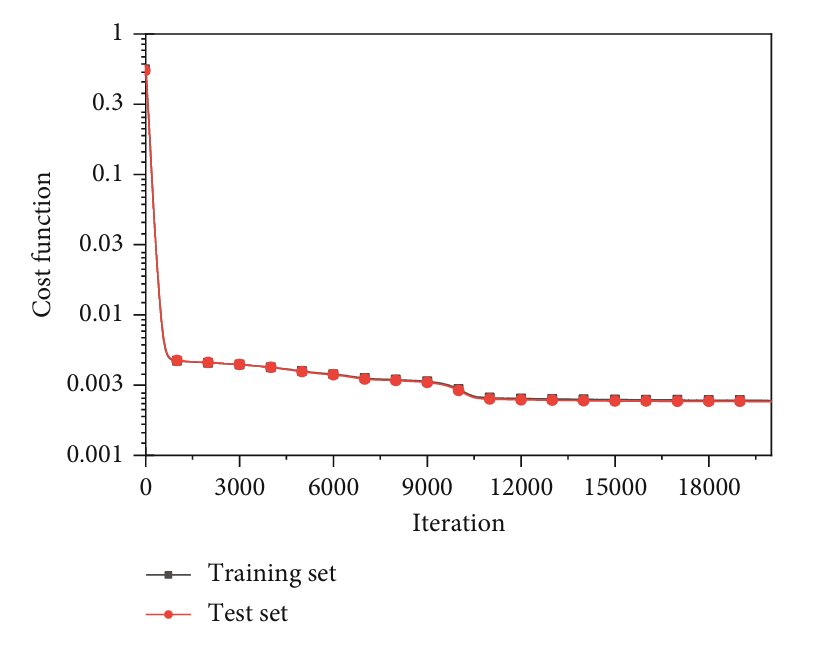
\includegraphics[width=0.55\linewidth]{Figures/17_nn_scf_convergence.png}
    \caption{Convergence curves of the NN-SCF loss function during training
             for different values of $\alpha$.
             All configurations converge within approximately 200 epochs.
             Reproduced from~\cite{zou2021novel}.}
    \label{fig:nnscf_convergence}
\end{figure}

\subsection{PAPR Reduction Performance}

\begin{figure}[H]
    \centering
    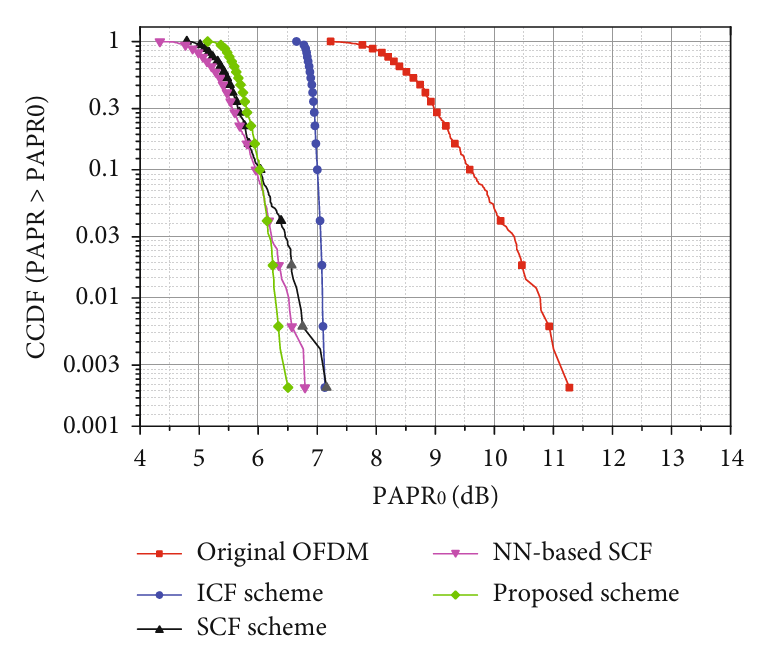
\includegraphics[width=0.55\linewidth]{Figures/18_nn_scf_ccdf.png}
    \caption{CCDF of PAPR for NN-SCF with different $\alpha$ values
             compared to original OFDM and conventional clipping.
             NN-SCF achieves 3--5~dB PAPR reduction depending on
             $\alpha$ at CCDF $= 10^{-3}$.
             Reproduced from~\cite{zou2021novel}.}
    \label{fig:nnscf_ccdf}
\end{figure}

\subsection{BER Performance}

\begin{figure}[H]
    \centering
    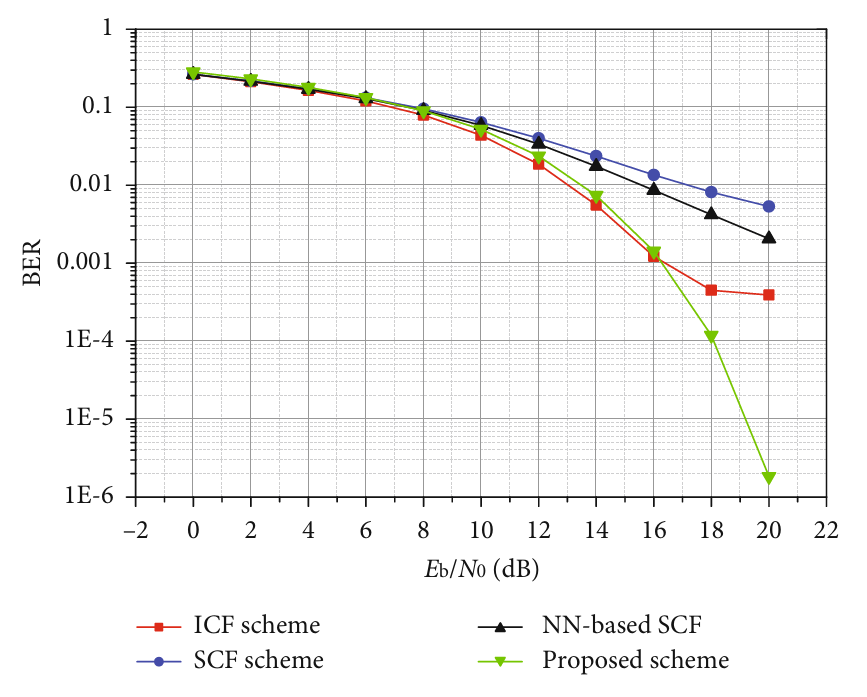
\includegraphics[width=0.55\linewidth]{Figures/19_nn_scf_ber.png}
    \caption{BER vs.\ SNR for NN-SCF compared to ICF and SCF schemes.
             NN-SCF achieves significantly better BER performance than traditional
             clipping-based methods while maintaining good PAPR reduction.
             Reproduced from~\cite{zou2021novel}.}
    \label{fig:nnscf_ber}
\end{figure}

\begin{figure}[H]
    \centering
    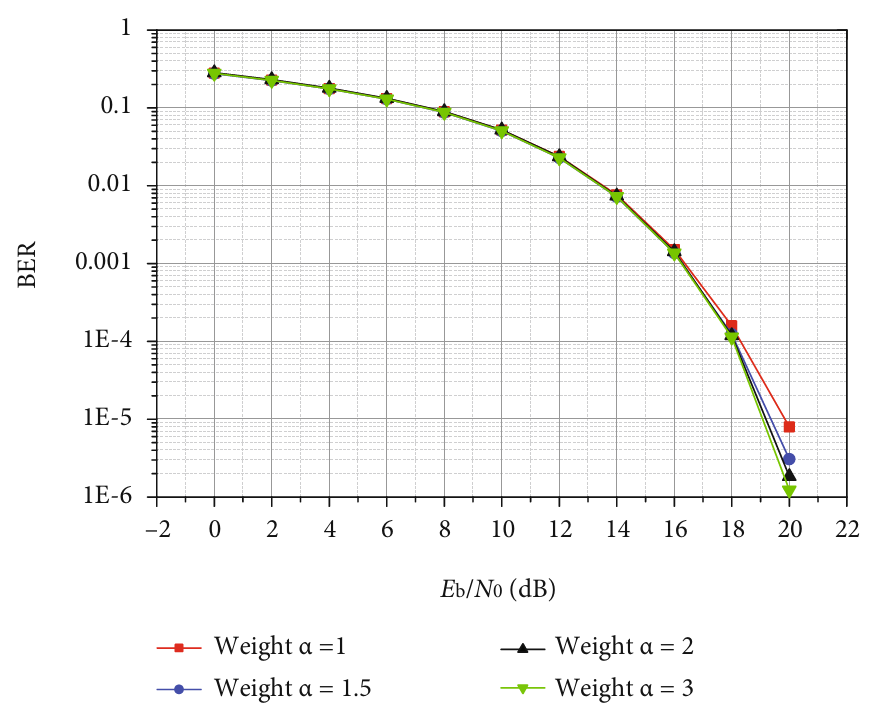
\includegraphics[width=0.55\linewidth]{Figures/20_nn_scf_ber_alpha.png}
    \caption{BER performance of NN-SCF under different weight parameter $\alpha$ values.
             Larger $\alpha$ (more emphasis on the recovery module) preserves
             BER performance better, while fitting the SCF scheme's PAPR reduction decreases.
             Reproduced from~\cite{zou2021novel}.}
    \label{fig:nnscf_ber_alpha}
\end{figure}


\subsection{Integration with Digital Pre-Distortion (DPD)}

\begin{figure}[H]
    \centering
    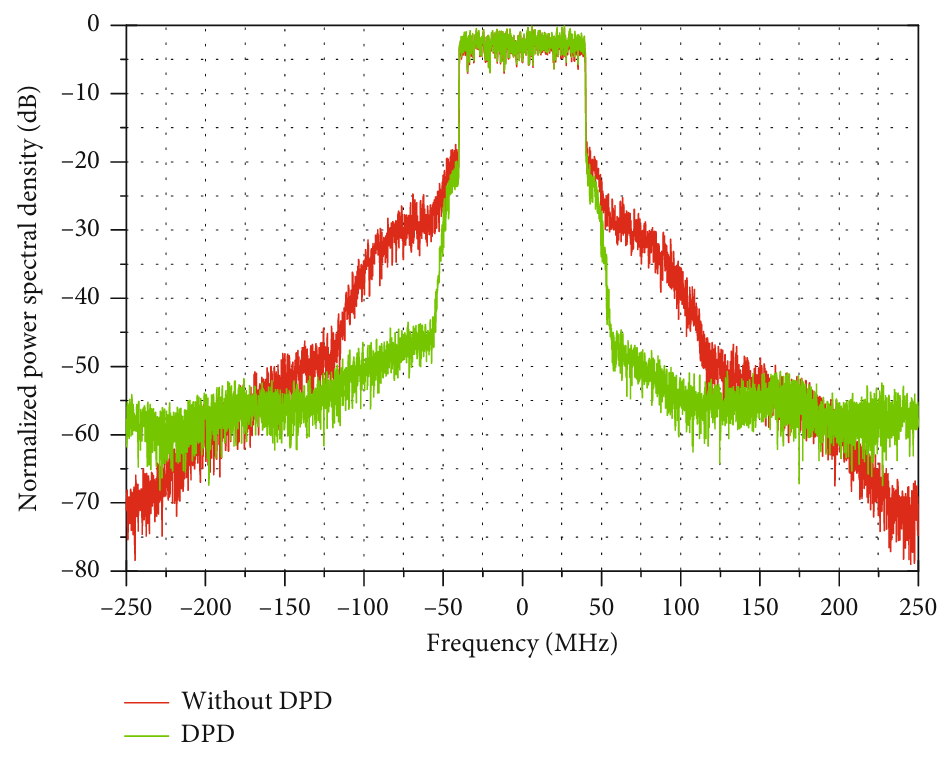
\includegraphics[width=0.55\linewidth]{Figures/21_nn_scf_psd_dpd.png}
    \caption{Normalized power spectral density (PSD) showing the linearization
             effect after performing Digital Pre-Distortion (DPD) on the
             low-PAPR signal generated by NN-SCF. The reduced PAPR enables
             the high-power amplifier to operate closer to saturation
             with significantly less out-of-band nonlinear distortion.
             Reproduced from~\cite{zou2021novel}.}
    \label{fig:nnscf_dpd}
\end{figure}


% ----------------------------------------------------------------------------
\section{Common Misconceptions}
\label{sec:nnscf_misconceptions}
% ----------------------------------------------------------------------------

\begin{misconception}
    \textbf{``NN-SCF and PRNet are the same idea.''} \\
    While both use DNNs for PAPR reduction, the architectures are
    fundamentally different.  PRNet uses an autoencoder that
    \emph{replaces} the OFDM signal with a learned representation.
    NN-SCF \emph{adds} a cancellation signal to the original OFDM
    signal.  This means NN-SCF preserves the OFDM signal structure
    and can be combined with existing OFDM receivers, while PRNet
    requires a matched decoder~\cite{zou2021novel,kim2017novel}.
\end{misconception}


% ----------------------------------------------------------------------------
\section{Limitations and Open Problems}
\label{sec:nnscf_limitations}
% ----------------------------------------------------------------------------

\begin{enumerate}
    \item \textbf{AWGN-only evaluation:}
          Like PRNet, NN-SCF was tested only under AWGN conditions.
          Fading channels are not addressed~\cite{zou2021novel}.

    \item \textbf{Power increase:}
          Adding the cancellation signal $\bm{c}$ to $\bm{x}$
          increases the average transmitted power, which must be
          accounted for in fair comparisons~\cite{zou2021novel}.

    \item \textbf{Two-module complexity:}
          The framework requires two separate DNNs (at transmitter and
          receiver), both of which must be deployed.

    \item \textbf{No side information formulation:}
          While NN-SCF avoids explicit SLM-style SI,
          the receiver must know the recovery module's parameters,
          which are agreed upon offline.
\end{enumerate}


% ----------------------------------------------------------------------------
\section{Connection to Other Approaches}
\label{sec:nnscf_connections}
% ----------------------------------------------------------------------------

NN-SCF extends the DNN-for-PAPR paradigm established by PRNet with two
key innovations~\cite{zou2021novel}:
\begin{itemize}
    \item The \textbf{signal cancellation} framework, which is more
          interpretable than the autoencoder approach and preserves
          the OFDM signal structure.
    \item The explicit \textbf{$\alpha$-parameterized trade-off},
          giving system designers a single knob to tune PAPR vs.\ BER.
\end{itemize}

The GA-SLM approach in the next chapter (Chapter~\ref{ch:ga_slm})
takes a completely different path: instead of learning a neural
transformation, it uses an evolutionary algorithm to directly search
for optimal SLM phase sequences~\cite{ali2016new}.
